\chapter{Bin Centering Corrections}
\label{cha:BCC}
%
When the cross-section is measured in 5-dimensional bins of $x$, $Q^2$, $z$, $P_{h\perp}^2$, and $\phi_h$, the result is the cross-section averaged over the phase space coverage of each bin (see figure~\ref{fig:BCC_basicExample}).
A more desirable quantity is the cross-section at the center point of the bin; therefore, bin centering corrections are applied.
%
\begin{figure}[htp]
\centering
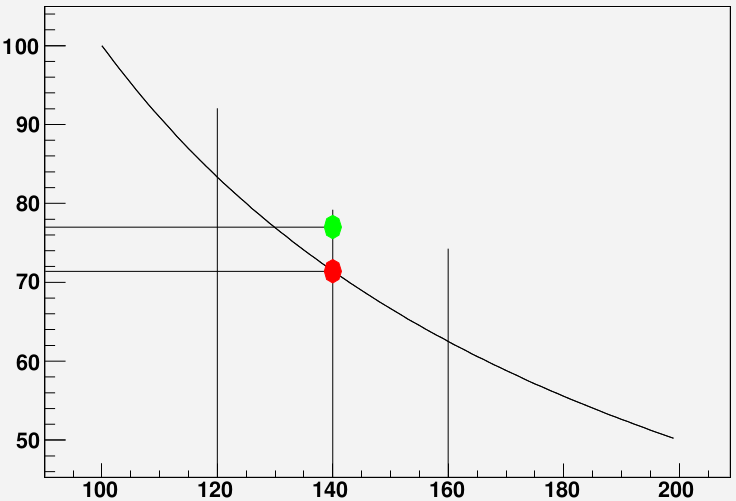
\includegraphics[width=3in]{figures/BCC_basicExample.png}
\caption{An example illustrating that the center point of a function (red point) can differ from the average value (green point).}
\label{fig:BCC_basicExample}
\end{figure}

Bin centering corrections are approximated using a model based on the results of the measurement.
Using the model, the cross-section is calculated in ``micro-bins'' (bins much smaller than the bins used for the final analysis, referred to here as ``normal bins''), the bin centering correction factor for a particular normal bin is then given by
\begin{equation}
\label{eq:BCCequation}
BCC\ factor = \frac{v}{V} \frac{\sigma_{averaged}}{\sigma_{center}}
\end{equation}
where $v$ is the 5-dimensional ``volume'' of the micro-bin at the center of the normal bin, $V$ is the volume the normal bin, $\sigma_{averaged}$ is the cross-section averaged over the normal bin, and $\sigma_{center}$ is the cross-section at the micro-bin at the center of the normal bin.

The micro-binning scheme is as follows: 90 $z$ bins from 0.0-0.9, 100 $P_{h\perp}^2$ bins 0.0-1.0 $GeV^2$, 50 $x$ bins from 0.1-0.6, 50 $Q^2$ bins from 1.0-5.0 $GeV^2$, 180 $\phi_h$ bins from -180-180 degrees.

\clearpage
